\section{Digital vs. Analog}

\subsection{Analog}
	\begin{compactitem}
		\item Die reale Welt ist analog (z.B. Sinnesorgane)
		\item Die analoge Verarbeitung stellt das Ergebnis einer Berechnung praktisch sofort zur Verf�gung.
		\item Analoge Systeme sind anf�llig auf externe St�rsignale.
		\item Analoge Systeme sind extrem aufw�ndig und erfordern viel Fachwissen.	
	\end{compactitem}
	
\subsection{Digital}
	\begin{compactitem}
		\item Einfacher automatisierbarer Entwurf und Test mit Hilfe von CAD m�glich.
		\item Digitale Schaltungen werden als integrierte Schaltungen mit Transistoren hergestellt uns sind somit reproduzierbar.
		\item Digitale Systeme sind bis zu einem gewissen Grad weitgehend immun gegen St�rsignale.
	\end{compactitem}
	
\subsection{Unterschied Analog zu Digital}
\begin{multicols}{3}
	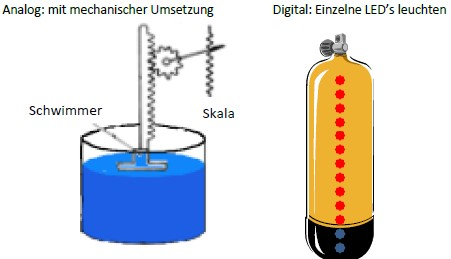
\includegraphics[width=5cm]{pics/unterschied_analog_digital.jpg}
		\columnbreak
	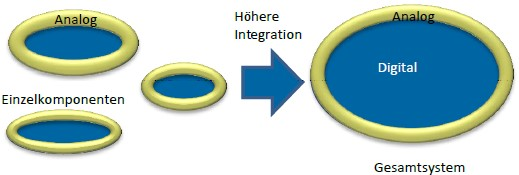
\includegraphics[width=5cm]{pics/analog_digital_integration.jpg}
		\columnbreak
		\\
	Trend zu h�herer Integration: Der digitale Anteil w�chst, wobei der analoge Teil weiterhin die Verbindung nach Aussen darstellt \lbrack wie eine Schale\rbrack.
\end{multicols}

%	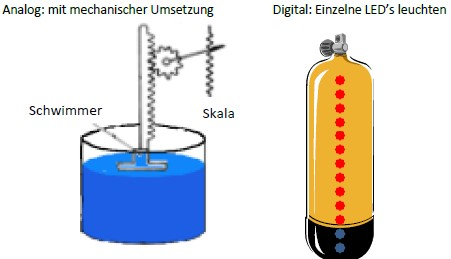
\includegraphics[width=0.3\textwidth]{pics/unterschied_analog_digital.jpg}
%	
%	\subsubsection{Integration}
%		\begin{minipage}[c]{8 cm}
%			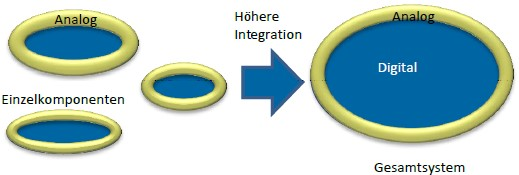
\includegraphics[width=0.9\textwidth]{pics/analog_digital_integration.jpg}
%		\end{minipage}
%		\begin{minipage}[c]{10 cm}
%			Trend zu h�herer Integration: Der digitale Anteil w�chst, wobei der analoge Teil weiterhin die Verbindung nach Aussen darstellt \lbrack wie eine Schale\rbrack.
%		\end{minipage}
%		
\subsection{Von Analog zu Digital}
	\begin{minipage}[c]{5 cm}
		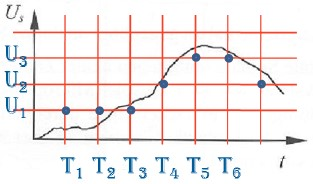
\includegraphics[width=0.9\textwidth]{pics/von_analog_zu_digital.jpg}
	\end{minipage}
	\begin{minipage}[c]{13 cm}
		\begin{minipage}[c]{4 cm}
			Abtasttheorem:
			\newline\newline\newline
			Amplitudenaufl�sung:
			\newline\newline\newline\newline\newline\newline
			Quantisierungsfehler:
			\newline
		\end{minipage}
		\begin{minipage}[c]{9 cm}
			Nyquist-Shannon besagt, dass ein Signal mit $f_{max}$ mit mindestens einer Frequenz von $2*f_{max}$ abgetastet werden muss, um das Ursprungssignal wieder herzustellen.\\
			Die Anzahl abz�hlbarer Amplitudenwerte (Quantisierungsstufen) bestimmt die Aufl�sung eines AD-Wandlers. Diese wird in der Regel in Bits angegeben. Je kleiner der Bereich aufgeteilt ist, desto kleiner ist der Abstand $\Delta A$ zwischen zwei benachbarten Amplitudenwerten.\\
			Anz. Quantisierungsstufen: $n_{q} = \frac{V_{max} - V{min}}{\Delta A} =$ n \\
			Bei linearer Quantisierung ist der Quantisierungsfehler (Quantisierungsrauschen) max. $\frac{\Delta A}{2}$	
		\end{minipage}
	\end{minipage}